%\documentclass[dvipdfmx]{beamer}      % platex の場合
\documentclass{beamer}                 % lualatex の場合
\usepackage{mySld}
\usepackage{multirow}

\begin{document}
\title{基礎コンピュータ工学\\第2章 情報の表現\\(パート5)}
\date{}

\begin{frame}
  \titlepage
\end{frame}

%==============================================================================
%\begin{frame}
%  \frametitle{}
%\end{frame}

\section{情報の表現}
%==============================================================================
\begin{frame}
  \frametitle{コンピュータの基本回路}
  \emph{論理回路}を組合せてコンピュータは製作される.
  \begin{itemize}
  \item 電気のOFFとONだけ用いて情報を表現する.
  \item \emph{OFF/ON}をビット\emph{0/1}に対応付ける.
  \item これは\emph{論理値}(True/False,真/偽,Yes/No)と同じ.
  \item 論理値を対象とする演算を\emph{論理演算}と言う.
  \item 論理演算を計算する回路を\emph{論理回路}と言う。
  \end{itemize}
  \vfill
  \centerline{論理IC => 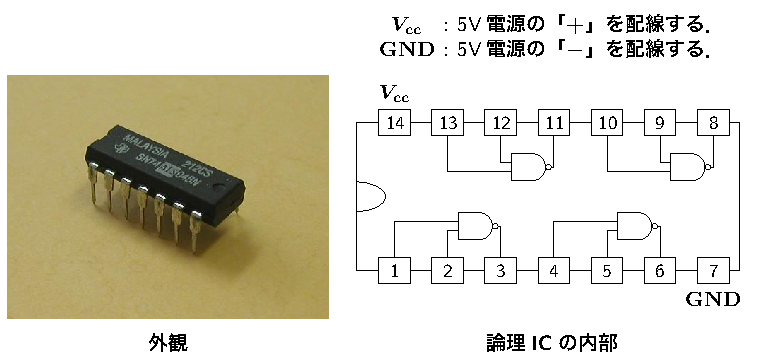
\includegraphics[scale=1.0]{../chap2/lic.pdf}}
\end{frame}

%==============================================================================
\begin{frame}
  \frametitle{論理ICで作った手作りコンピュータ}
  \emph{徳山高専卒業研究}で約30年前に製作された手作りコンピュータ
  \vfill
  \begin{tabular}{c c}
  \multirow{2}{*}{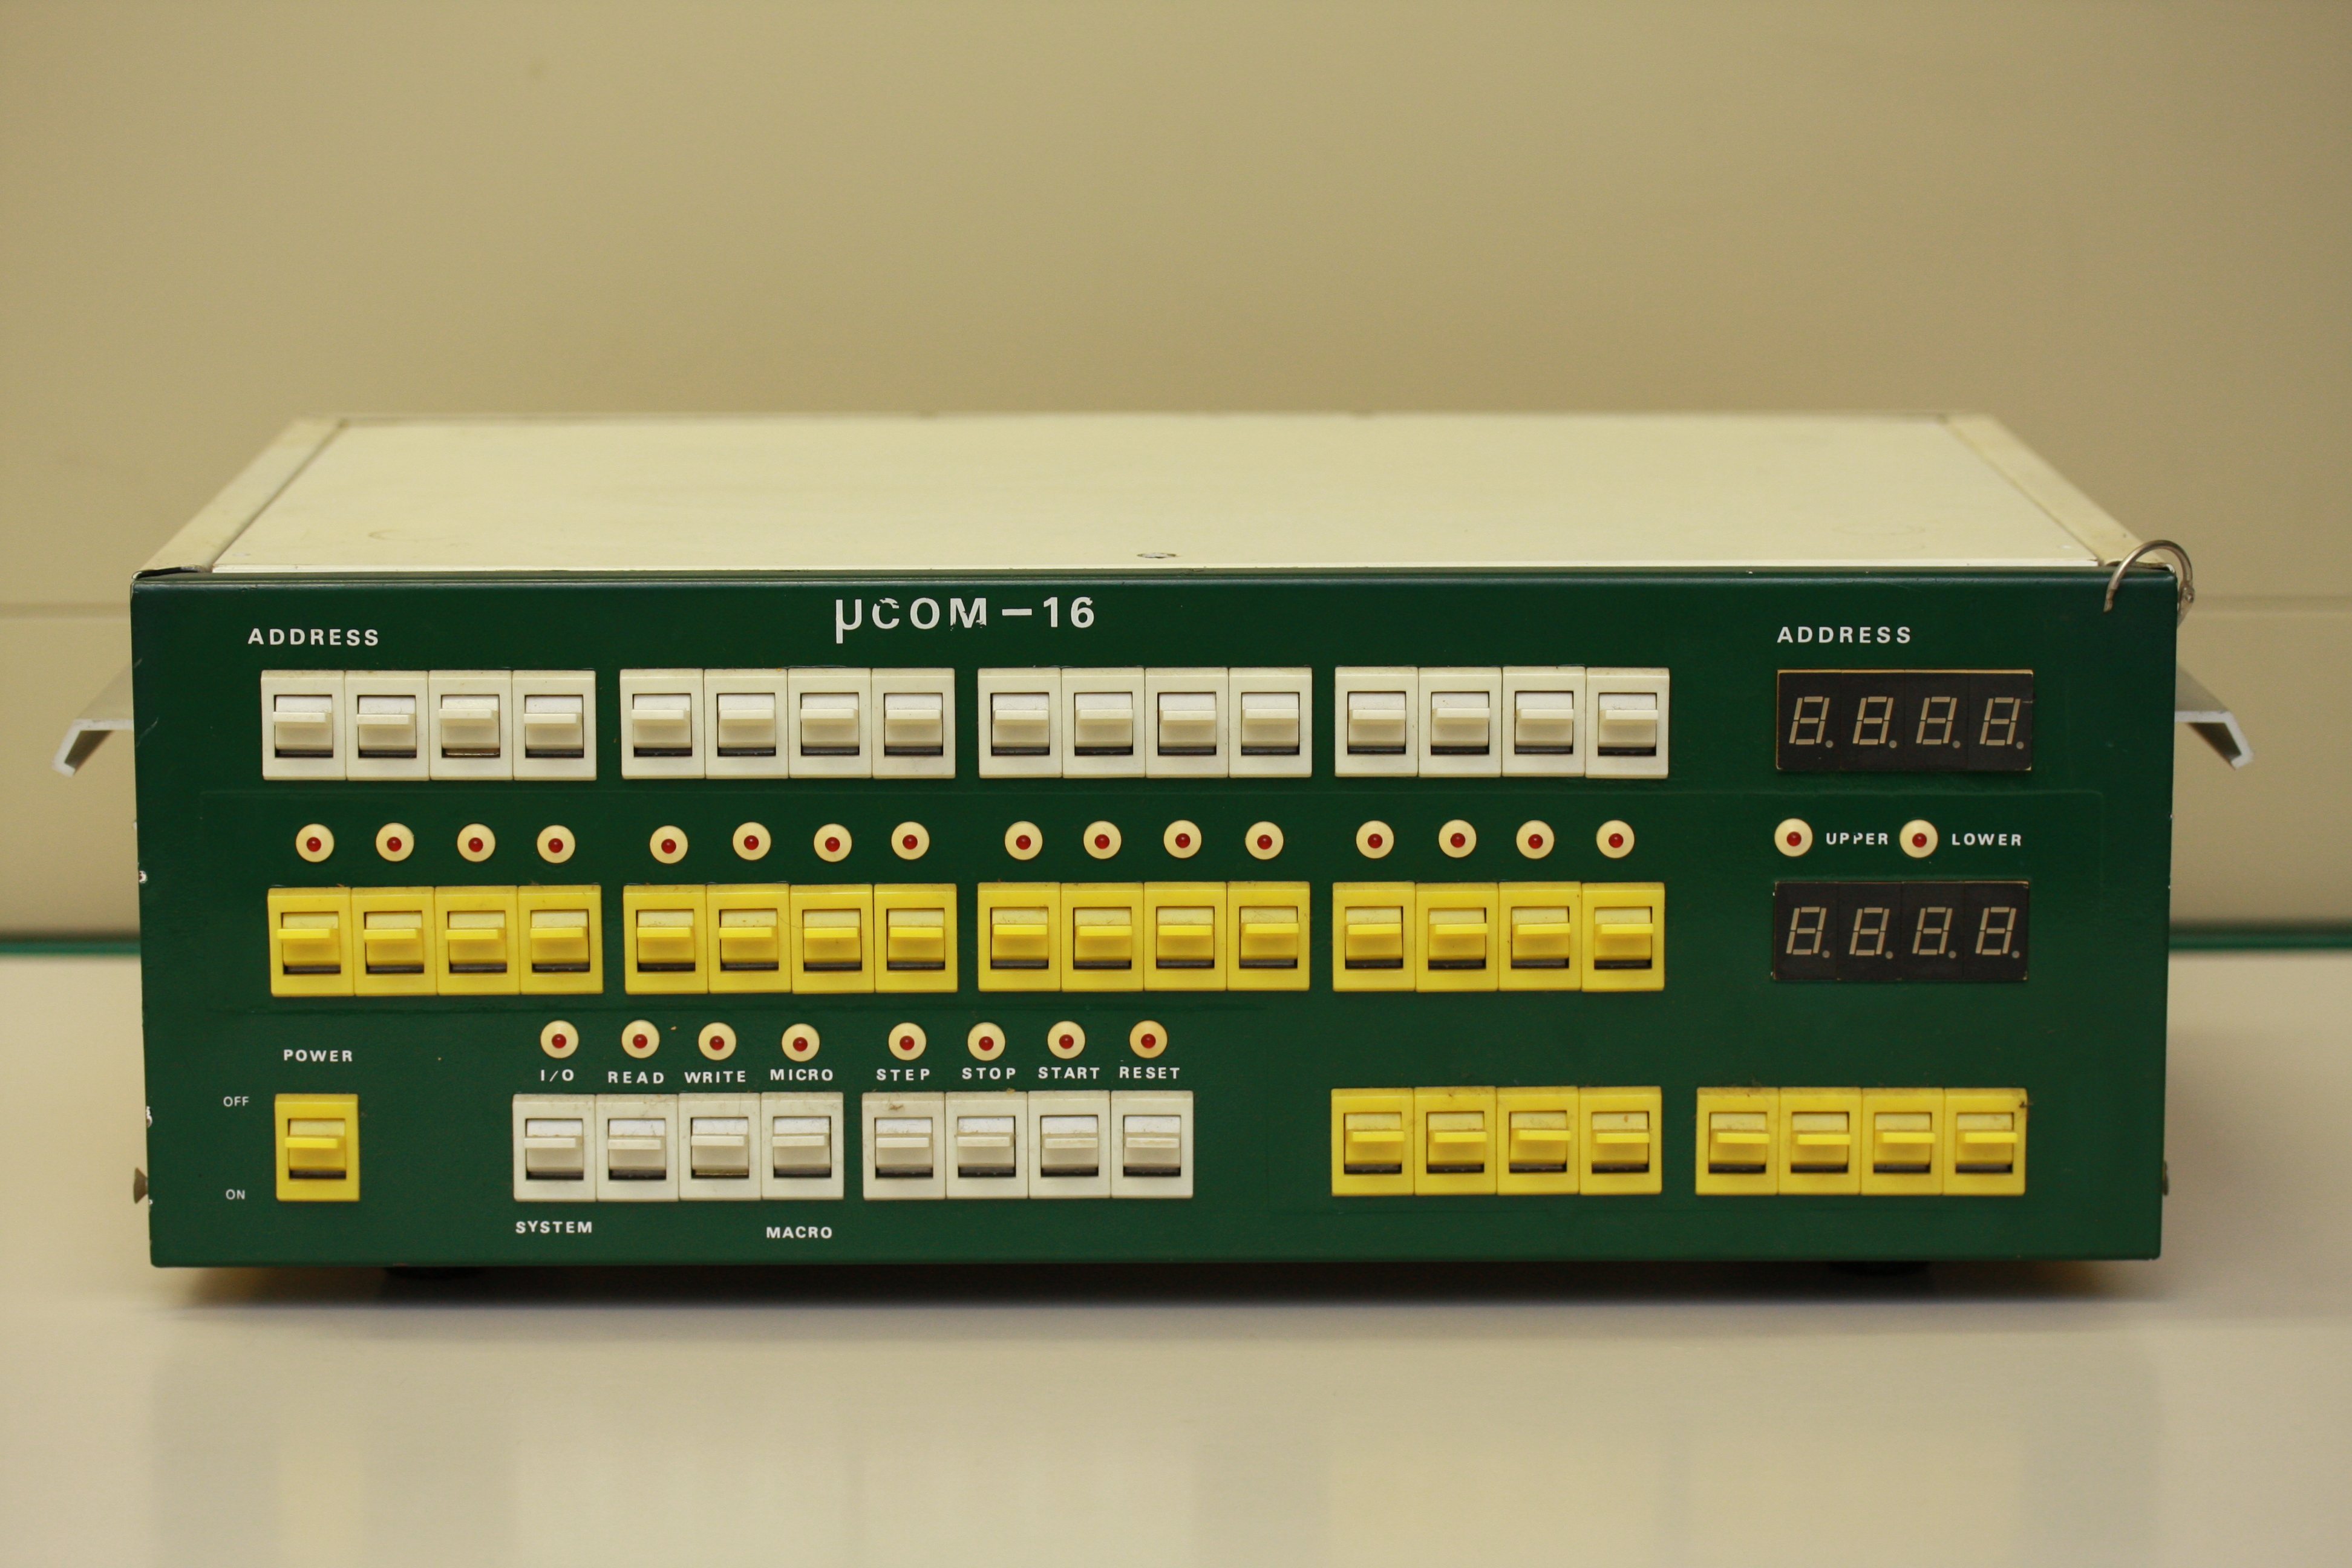
\includegraphics[scale=0.04]{../chap2/uCom16_1.jpg}}
  &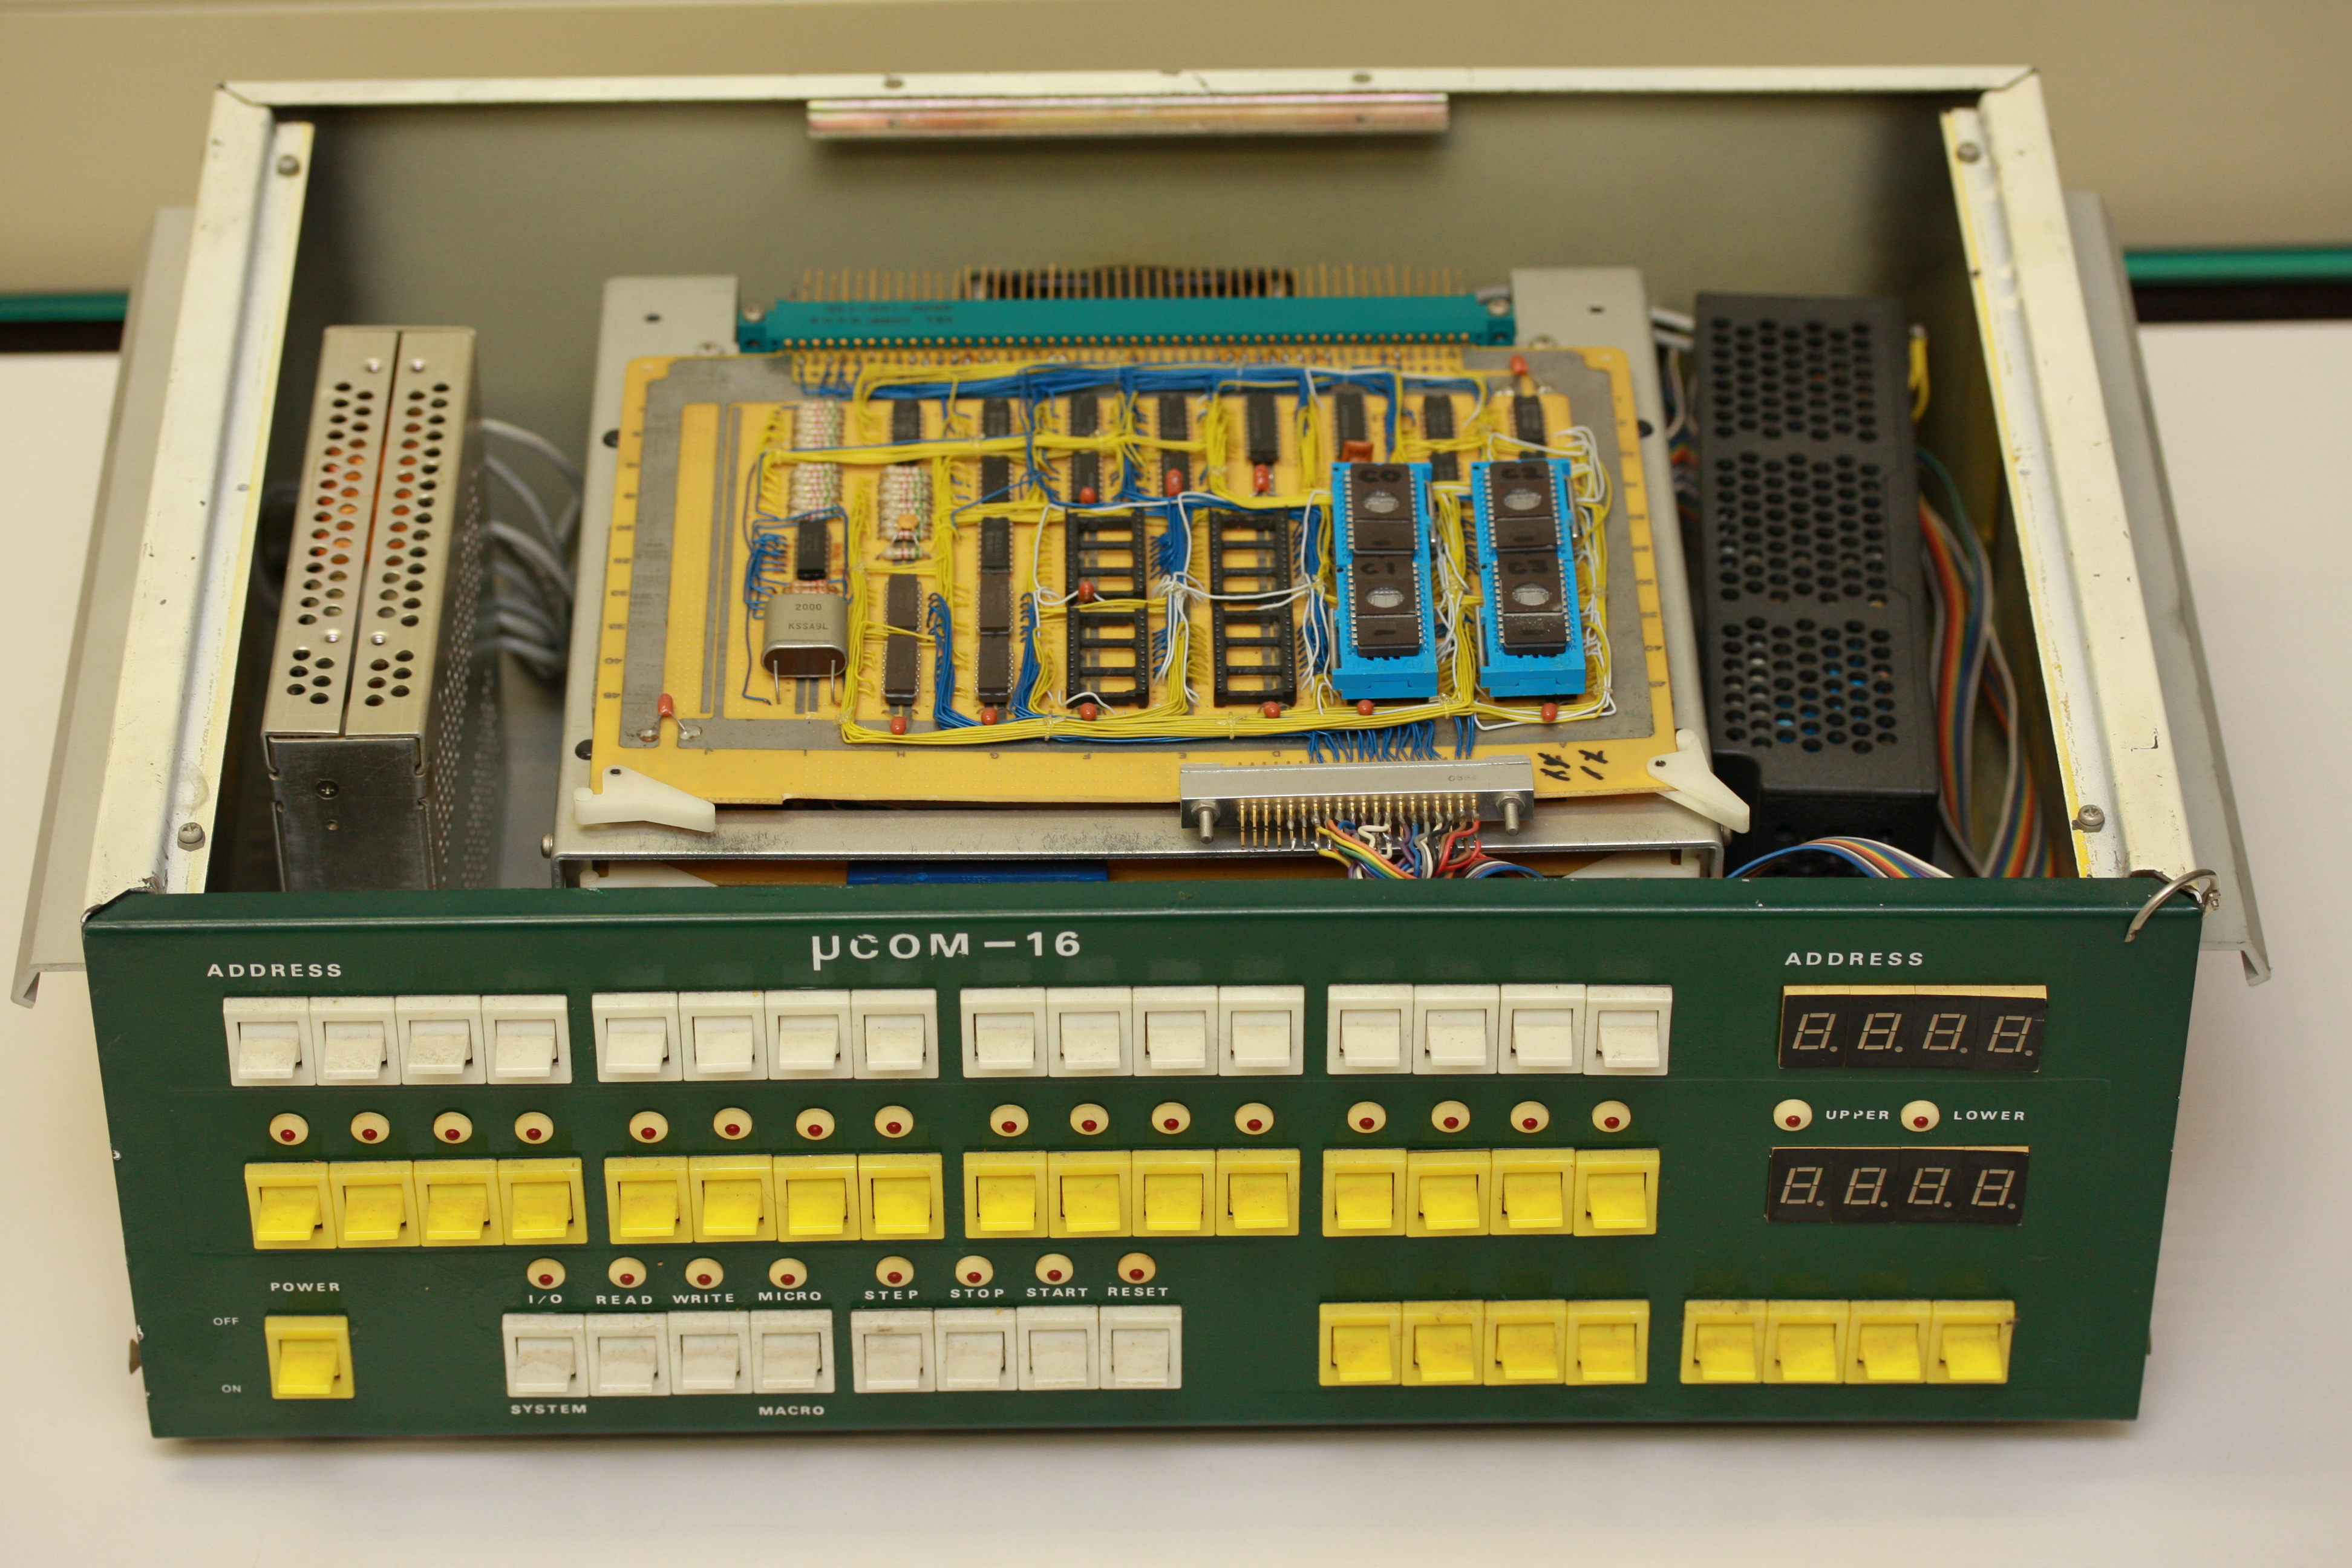
\includegraphics[scale=0.03]{../chap2/uCom16_2.jpg} \\
  &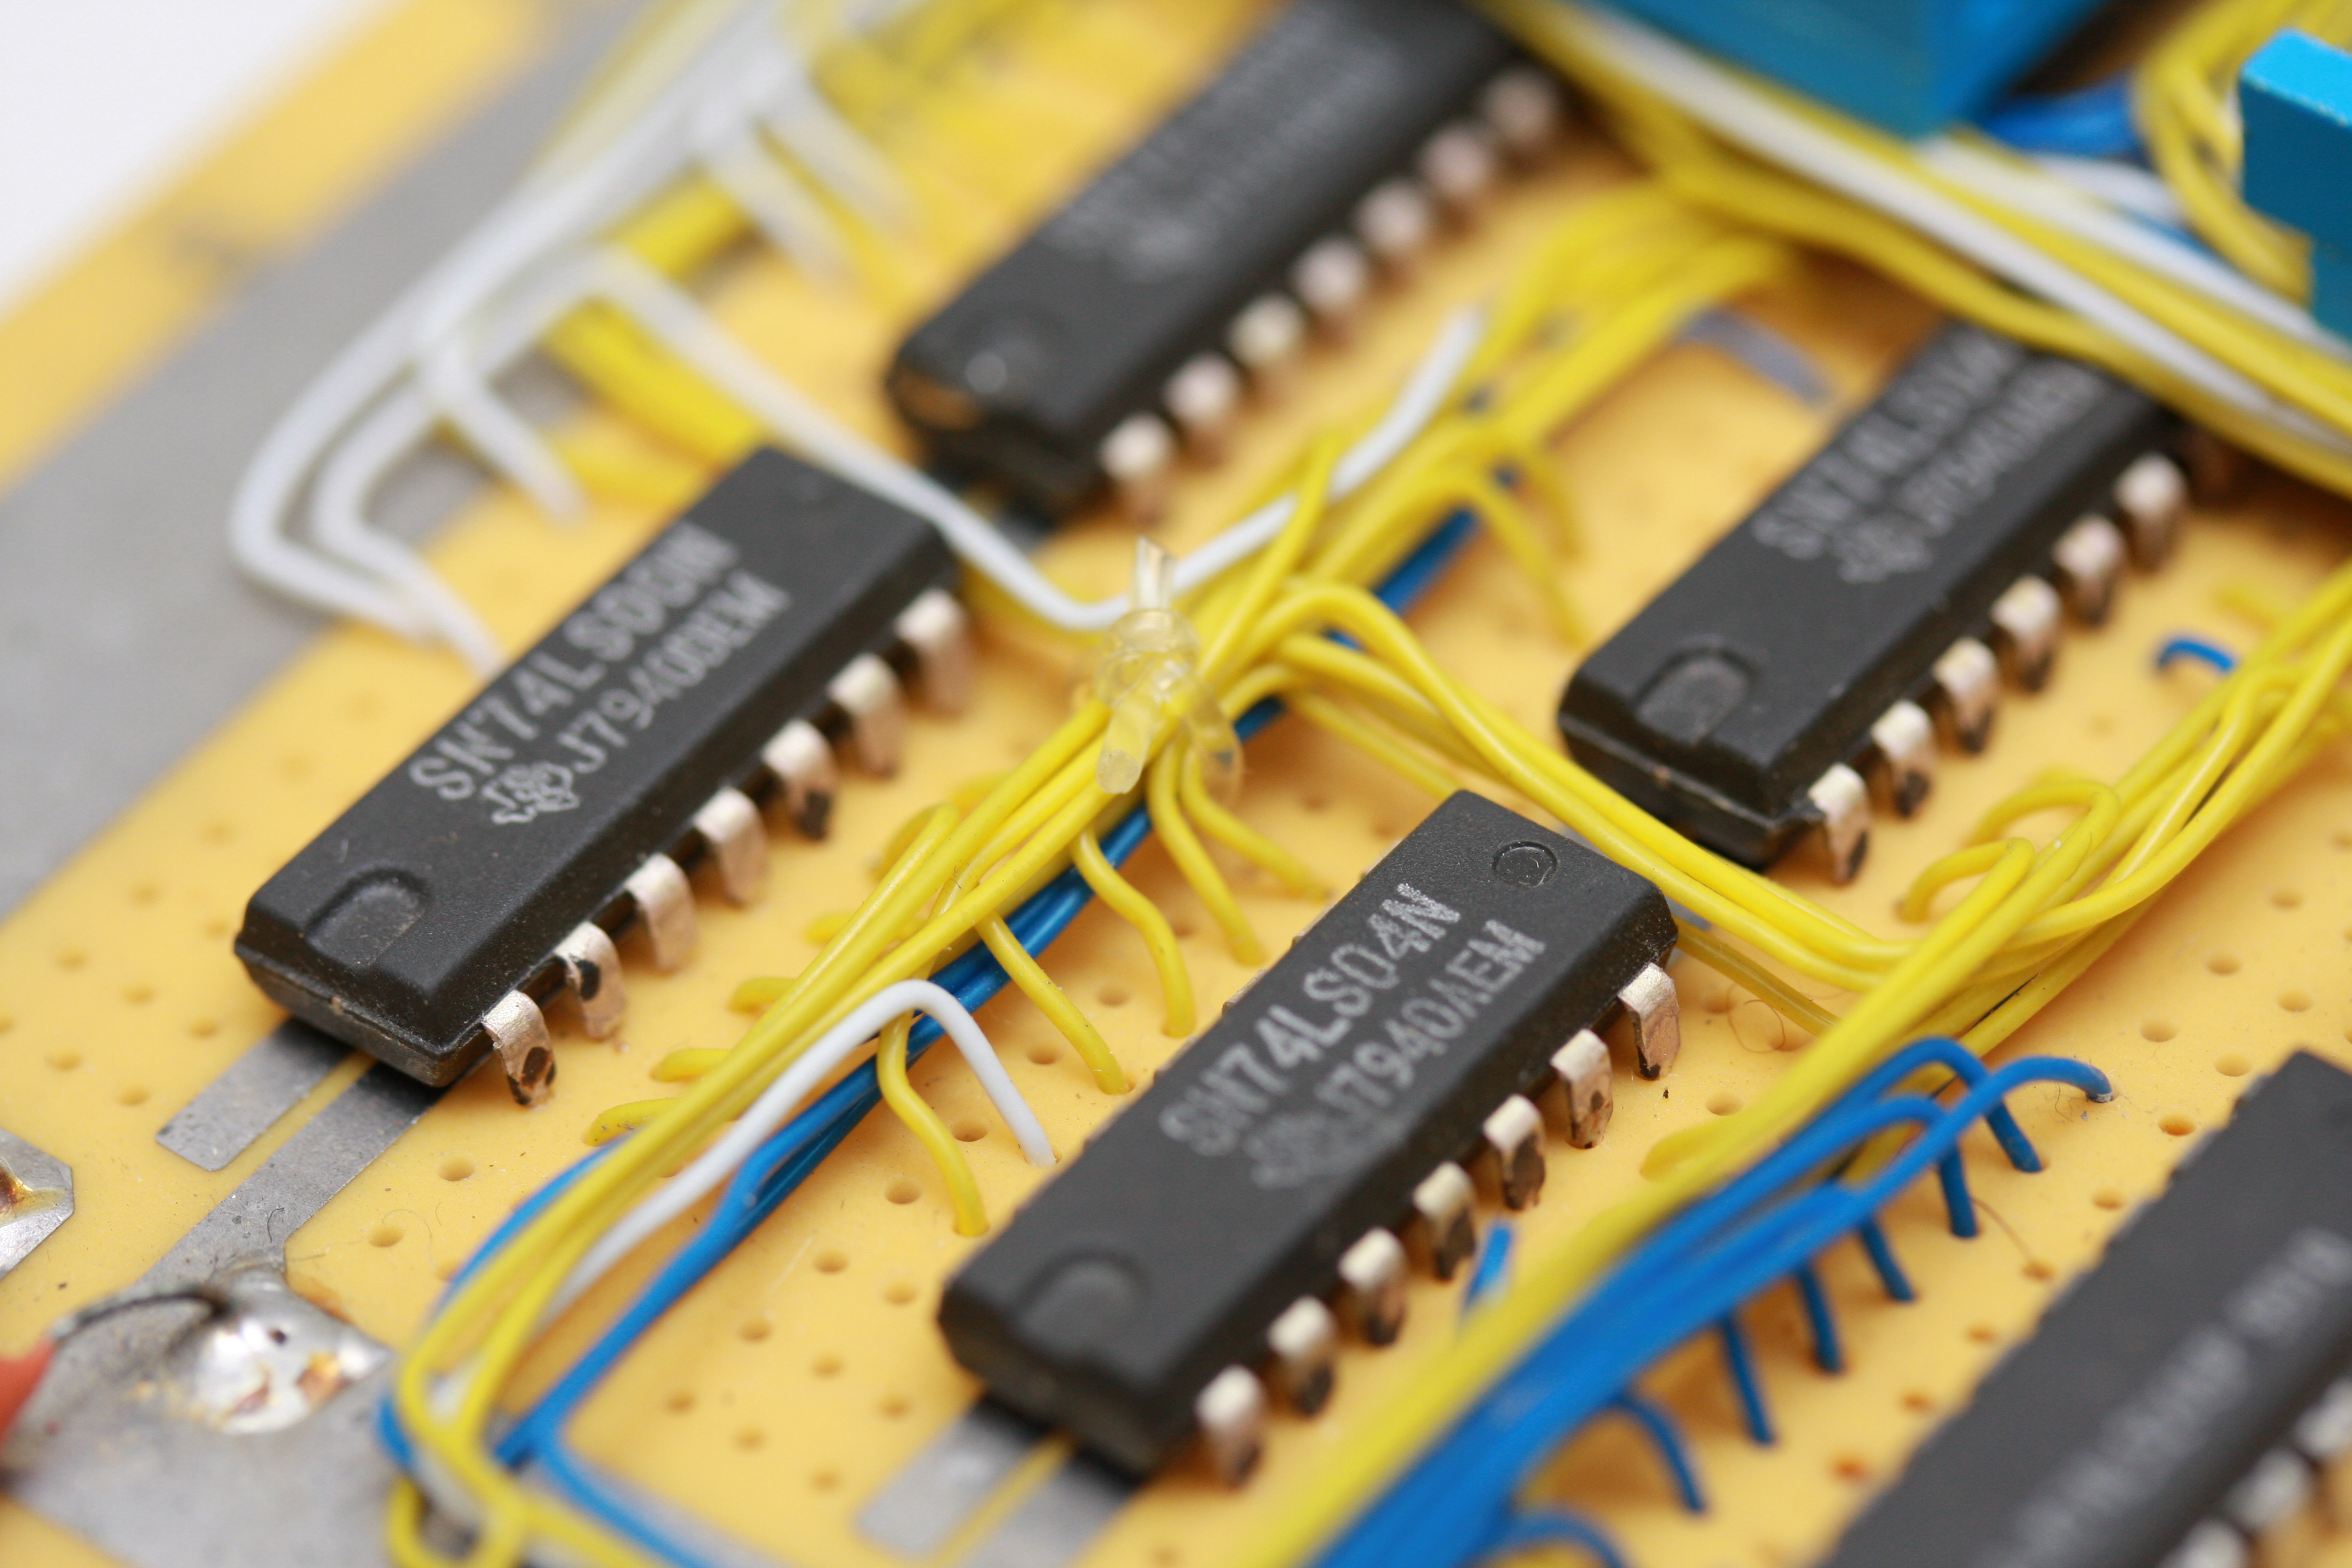
\includegraphics[scale=0.03]{../chap2/uCom16_3.jpg}
  \end{tabular}
\end{frame}

%==============================================================================
\begin{frame}
  \frametitle{論理ICで回路を作る}
  \centerline{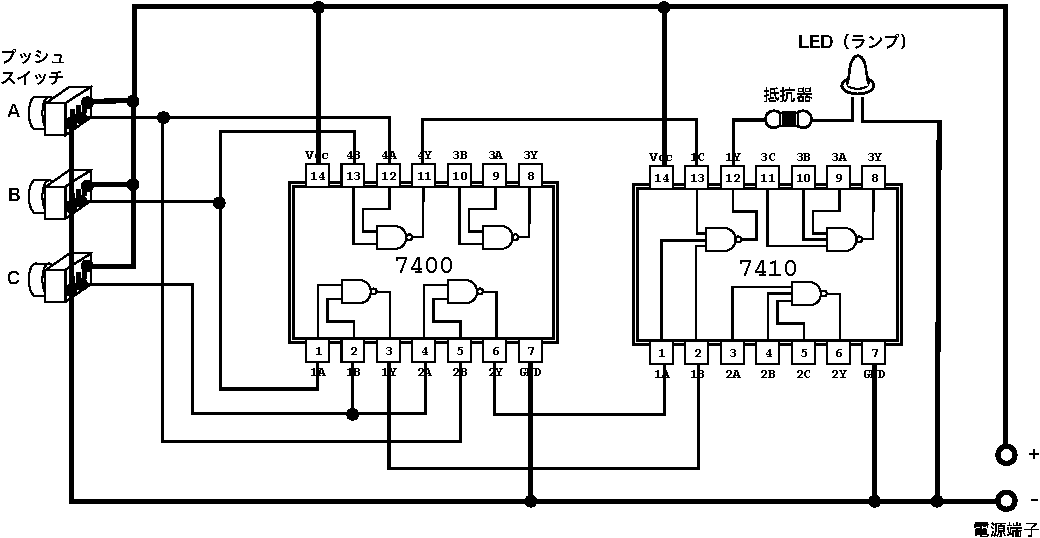
\includegraphics[scale=0.6]{../chap2/majority-crop.pdf}}
\end{frame}

%==============================================================================
\begin{frame}
  \frametitle{現代の手作りコンピュータ}
  \emph{FPGA}の中に論理IC数万個に相当する回路が書き込める.
  \vfill
  \centerline{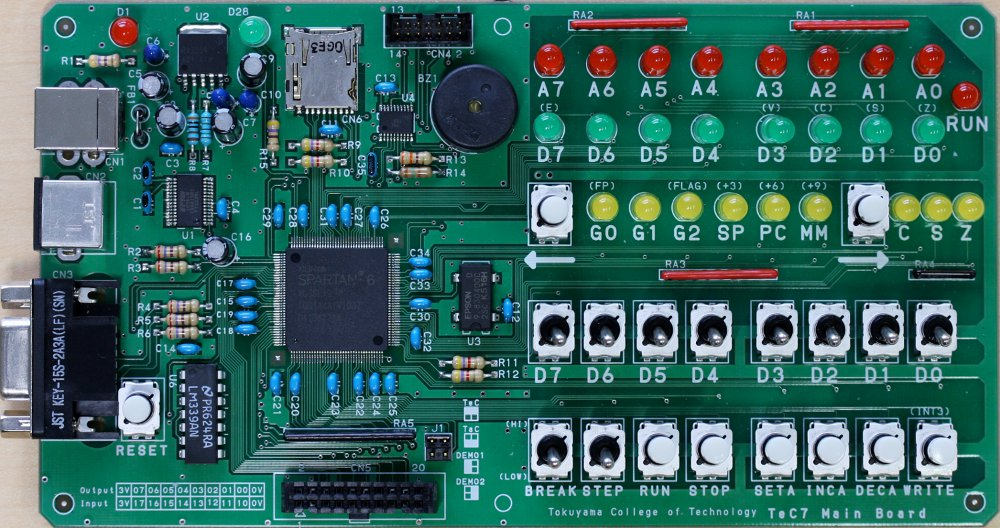
\includegraphics[scale=0.3]{../chap4/TeC7.jpg}}
\end{frame}

%==============================================================================
\begin{frame}
  \frametitle{基本的な論理回路(1)}
  \emph{論理積(AND)} --- 「かつ」\\
  \vfill
  2ビット入力し,両方が1のときだけ1を出力する.
  \begin{center}
    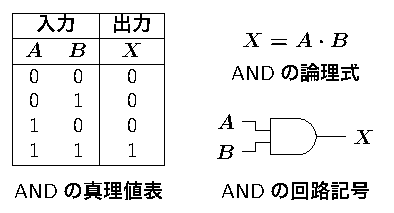
\includegraphics[scale=2.0]{../chap2/and.pdf}
  \end{center}
  \begin{quote}
    A \emph{かつ} B が1 なら 1\\
    A \emph{AND} B が1 なら 1
  \end{quote}
\end{frame}

%==============================================================================
\begin{frame}
  \frametitle{基本的な論理回路(2)}
  \emph{論理和(OR)} --- 「または」\\
  \vfill
  2ビット入力し,どちらかが1のとき1を出力する.
  \begin{center}
    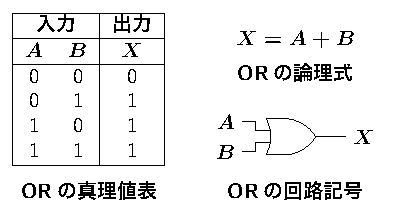
\includegraphics[scale=2.0]{../chap2/or.pdf}
  \end{center}
  \begin{quote}
    A \emph{または} B が1 なら 1\\
    A \emph{OR} B が1 なら 1
  \end{quote}
\end{frame}

%==============================================================================
\begin{frame}
  \frametitle{基本的な論理回路(3)}
  \emph{否定(NOT)} --- 「ではない」\\
  \vfill
  1ビット入力し,入力とは逆の論理値をを出力する.
  \begin{center}
    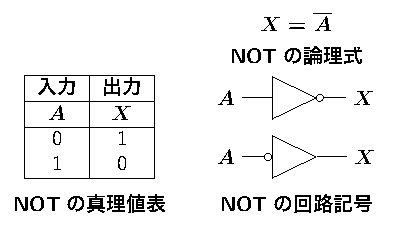
\includegraphics[scale=2.0]{../chap2/not.pdf}
  \end{center}
  \begin{quote}
    A が 1 \emph{ではない} なら 1\\
  \end{quote}
\end{frame}

%==============================================================================
\begin{frame}
  \frametitle{基本的な論理回路(4)}
  \emph{排他的論理和(XOR)} --- 「異なる」\\
  \vfill
  2ビット入力し,二つが異なるなら1を出力する.
  \begin{center}
    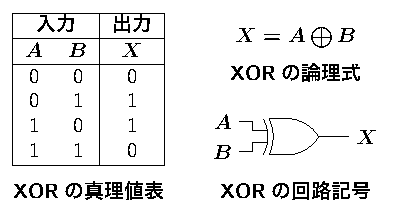
\includegraphics[scale=2.0]{../chap2/xor.pdf}
  \end{center}
  \begin{quote}
    A と B が異なるなら 1\\
  \end{quote}
\end{frame}

%==============================================================================
\begin{frame}
  \frametitle{基本的な論理回路(5)}
  \emph{NOTとANDの組合せ(NAND)} \\
  \vfill
  \begin{center}
    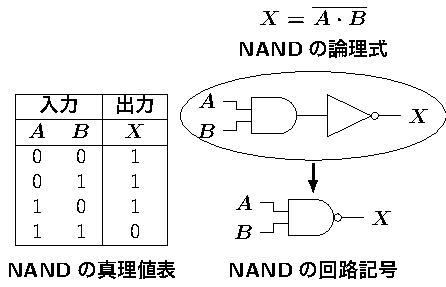
\includegraphics[scale=2.0]{../chap2/nand.pdf}
  \end{center}
\end{frame}

%==============================================================================
\begin{frame}
  \frametitle{基本的な論理回路(6)}
  \emph{NOTとORの組合せ(NOR)} \\
  \vfill
  \begin{center}
    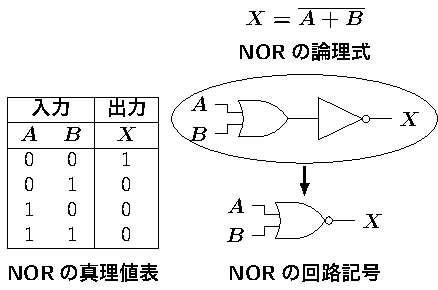
\includegraphics[scale=2.0]{../chap2/nor.pdf}
  \end{center}
\end{frame}

%==============================================================================
\begin{frame}
  \frametitle{演算回路(1)}
  \emph{半加算器} \\
  1桁の2進数を二つ入力し,0,1,2のどれかを出力する.
  \vfill
  \begin{center}
    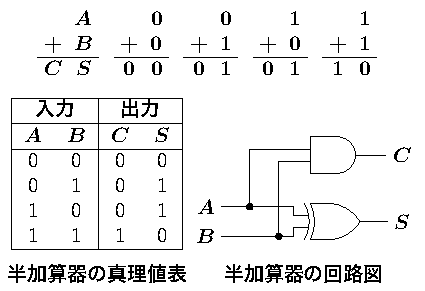
\includegraphics[scale=2.0]{../chap2/ha.pdf}
  \end{center}
\end{frame}

%==============================================================================
\begin{frame}
  \frametitle{演算回路(2)}
  \emph{全加算器} \\
  1桁の2進数を三つ入力し,0,1,2,3のどれかを出力する.
  \vfill
  \begin{center}
    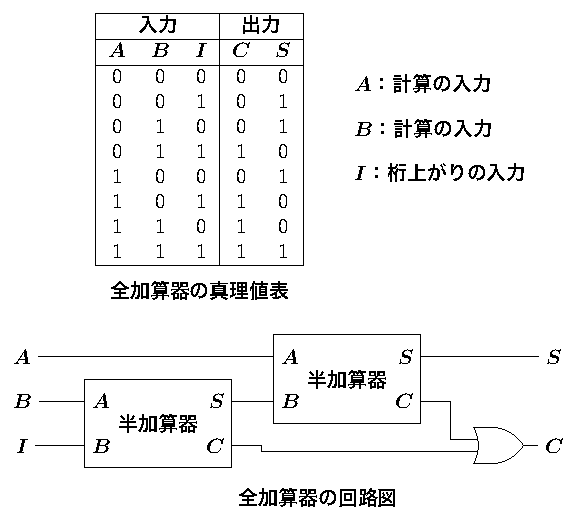
\includegraphics[scale=1.3]{../chap2/fa.pdf}
  \end{center}
\end{frame}

%==============================================================================
\begin{frame}
  \frametitle{演算回路(3)}
  \emph{4ビット加算器} \\
  4桁の2進数を二つ入力し,和を計算する
  \vfill
  \begin{center}
    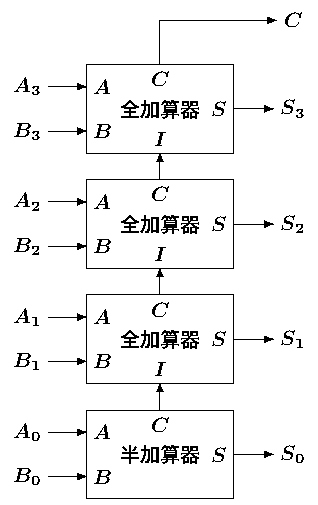
\includegraphics[scale=1.3]{../chap2/adder.pdf}
  \end{center}
\end{frame}

%==============================================================================
\begin{frame}
  \frametitle{演算回路(4)}
  \emph{4ビット 1の補数器} \\
  4桁の2進数を入力し,1の補数を計算する
  \vfill
  \begin{center}
    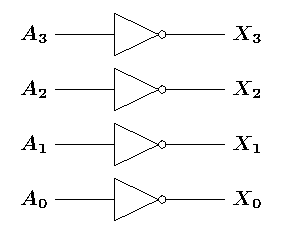
\includegraphics[scale=1.3]{../chap2/onesc.pdf}
  \end{center}
\end{frame}

%==============================================================================
\begin{frame}
  \frametitle{演算回路(5)}
  \emph{4ビット 2の補数器} \\
  4桁の2進数を入力し,2の補数を計算する
  \vfill
  \begin{center}
    \includegraphics[scale=1.3]{../chap2/towsc.pdf}
  \end{center}
\end{frame}

%==============================================================================
\begin{frame}
  \frametitle{記憶回路}
  \emph{RSフリップフロップ} \\
  直前の状態を記憶する回路
  \vfill
  \begin{center}
    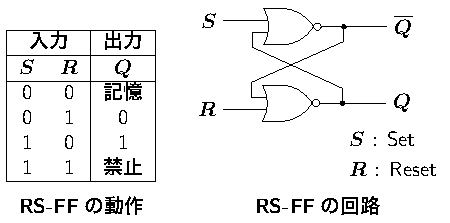
\includegraphics[scale=2.0]{../chap2/rsff.pdf}
  \end{center}
\end{frame}

\end{document}
